\section{Les algorithmes de calcul de distance}
% Un algorithme de calcul de distance permet de mesurer la similarité et/ou la dif-
% férence entre deux objets tels que du texte, des vecteurs, des chaînes de caractères.
% On utilise ces algorithmes de calcul principalement pour la correction d’orthographe,
% le traitement de texte, les alignements de séquences ADN ou encore pour la recherche
% d’information


\begin{frame}{Distance de Levenshtein}
	\textbf{Objectif : }Trouver le nombre minimal d'opérations nécessaires pour transformer une chaîne de caractères en une autre.
	\begin{center}
		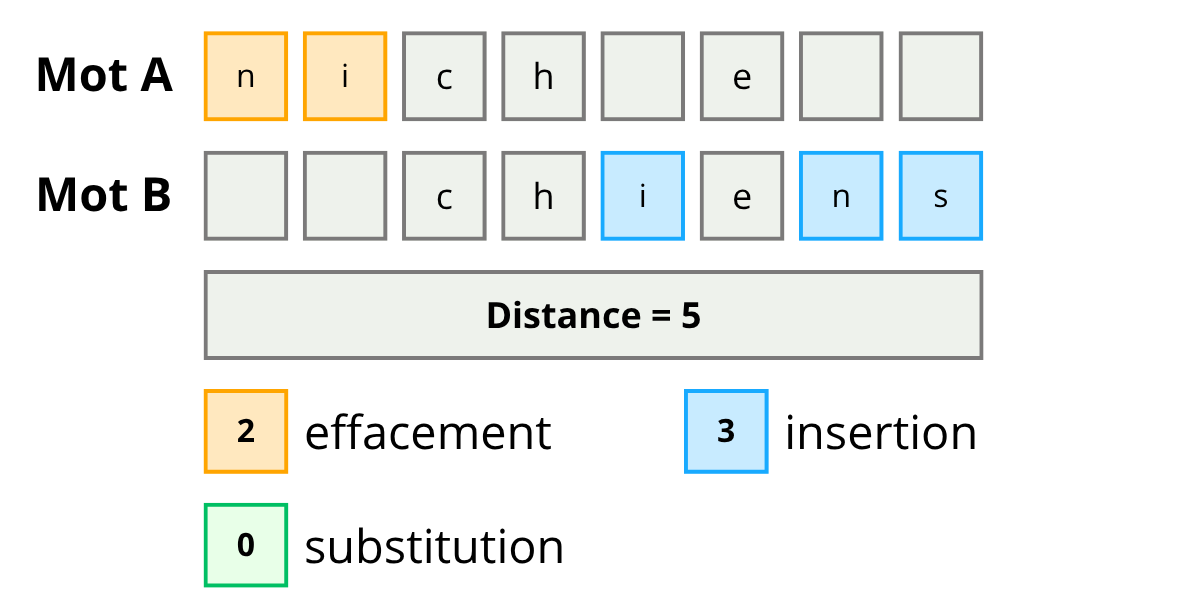
\includegraphics[width=0.9\textwidth]{images/levenshtein.png}
	\end{center}
	\textbf{Complexité : }  $\mathcal{O}(n \times m)$ (où n et m sont les longueurs des chaînes de caractères)
\end{frame}

\begin{frame}{Distance de Damerau-Levenshtein}
	\vspace*{-0.3cm}
	\textbf{Objectif : }identique à la distance de Levenshtein, mais avec l'ajout de la possibilité d'échanger deux caractères adjacents.
	\begin{center}
		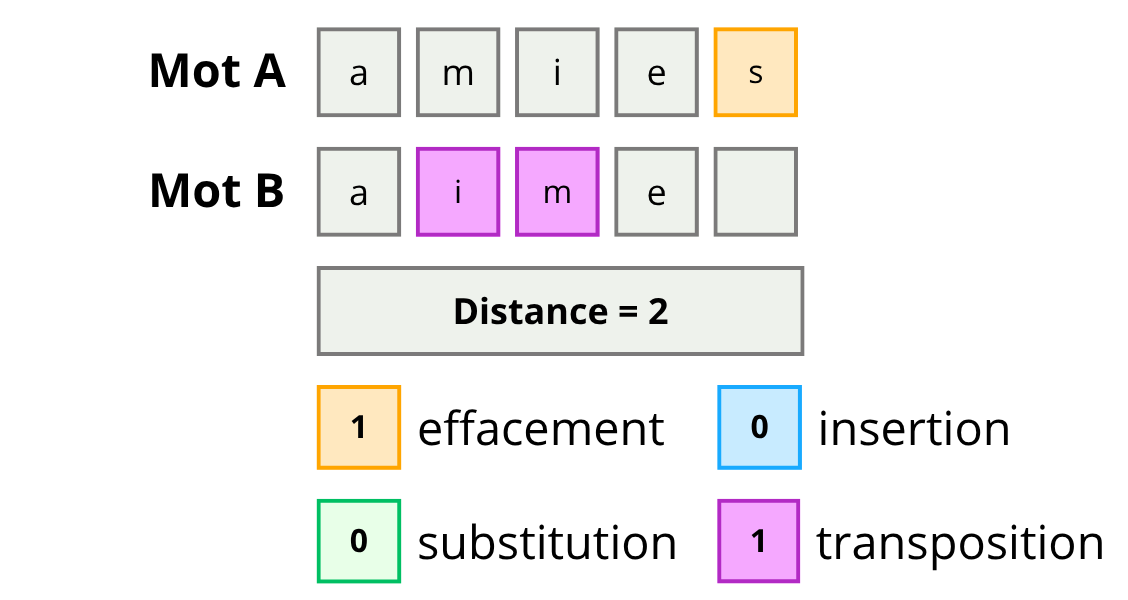
\includegraphics[width=0.9\textwidth]{images/damerau-levenshtein.png}
	\end{center}
	\textbf{Complexité : }  $\mathcal{O}(n \times m)$ (où n et m sont les longueurs des chaînes de caractères)
\end{frame}

\begin{frame}{Distance de Hamming}
	\begin{columns}
		\column{0.5\textwidth}
		Compter le nombre de positions où les caractères diffèrent.
		\column{0.5\textwidth}
		Utilisable que pour des mots de même longueur.
	\end{columns}
	\begin{center}
		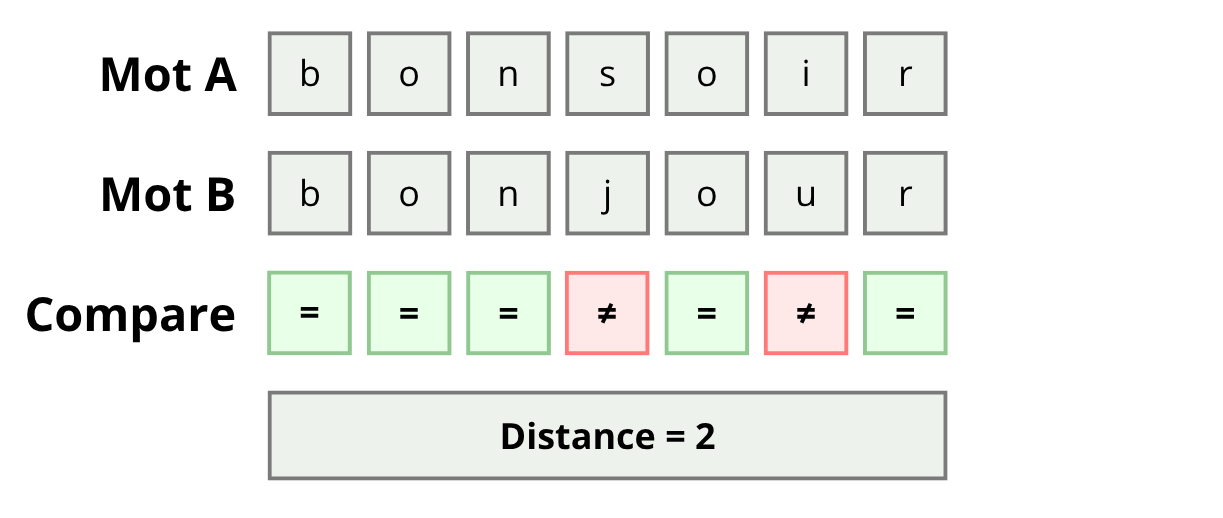
\includegraphics[width=0.9\textwidth]{images/hamming.png}
	\end{center}
	\textbf{Complexité : }  $\mathcal{O}(n)$ (où n est la longueur des chaînes de caractères)
\end{frame}
